\chapter{Expérience 2 : Projet Collaboratif Innovant - Développement d'un jeu vidéo interdisciplinaire}

\section{Axe 1 : Contexte et genèse du projet}

\subsection{Une solution créative à une contrainte institutionnelle}

Confronté à l'impossibilité de réaliser un Projet Collaboratif Innovant (PCI) classique en tant qu'unique stagiaire NSI de mon établissement (les PCI nécessitant normalement la collaboration entre plusieurs stagiaires), j'ai proposé à l'INSPÉ un projet intra-établissement impliquant plusieurs disciplines.

Cette proposition a été perçue par mes formateurs comme une \textbf{excellente initiative}, revenant à l'esprit originel du dispositif PCI : favoriser la collaboration interdisciplinaire et le décloisonnement des enseignements \parencite{referentiel_meef,projet_travail_groupe}.

\subsection{Objectifs pédagogiques transversaux}

L'objectif principal n'était pas uniquement technique (développer un jeu vidéo), mais visait surtout le développement de \textbf{compétences transversales} essentielles au XXIe siècle \parencite{competences_transversales_eurecia,competences_21_siecle}:

\begin{itemize}[leftmargin=*]
    \item \textbf{Travail d'équipe} : collaboration entre élèves de niveaux et profils différents
    \item \textbf{Gestion de projet} : respect des contraintes (délais, ressources), planification, coordination
    \item \textbf{Communication interdisciplinaire} : articulation entre compétences techniques (code), créatives (graphisme, musique), narratives (scénario) et linguistiques (traduction)
    \item \textbf{Résolution de problèmes complexes} : décomposition d'un projet ambitieux en sous-tâches gérables
\end{itemize}

Ces compétences sont au cœur de la pédagogie par projet préconisée par les programmes NSI \parencite{projet_methode_tlem,nsi_programmes}.

Analysée à travers le \textbf{triangle pédagogique de Jean Houssaye} \parencite{houssaye_triangle}, cette séquence marque un déplacement délibéré des processus en jeu :
\begin{itemize}[leftmargin=*]
    \item La phase initiale de cours relevait du processus \textbf{« Enseigner »} (relation Professeur-Savoir).
    \item La phase de projet bascule vers les processus \textbf{« Former »} (Professeur-Élève, par l'accompagnement) et surtout \textbf{« Apprendre »} (Élève-Savoir), où l'élève construit son savoir par l'action.
\end{itemize}

De plus, la \textbf{transposition didactique} \parencite{chevallard_transposition} opérée ici est spécifique : le savoir savant (la programmation orientée objet, les vecteurs mathématiques) n'est pas scolarisé sous forme d'exercices académiques, mais transformé en outils fonctionnels pour la création. Le code « expert » du moteur de jeu (Pygame) a été didactisé (apprêté) pour être accessible aux élèves, leur permettant de manipuler des concepts complexes sans être noyés par la complexité technique sous-jacente.

\subsection{Support stratégique : le jeu vidéo comme vecteur de motivation}

Le jeu vidéo a été choisi pour plusieurs raisons pédagogiques stratégiques \parencite{pedagogie_active} :

\begin{enumerate}[leftmargin=*]
    \item \textbf{Motivation intrinsèque} : Le jeu vidéo est un domaine familier et attractif pour les lycéens, générant un engagement spontané
    \item \textbf{Complexité technique maîtrisable} : Un jeu 2D en Python/Pygame permet d'aborder tous les concepts du programme NSI (POO, structures de données, algorithmique, gestion d'événements) sans nécessiter de connaissances trop avancées
    \item \textbf{Production valorisante} : Un jeu fonctionnel constitue une réalisation concrète et partageable, source de fierté pour les élèves
    \item \textbf{Préparation aux Olympiades de NSI} : Le projet s'inscrivait dans une perspective d'excellence, entraînant les élèves à un projet ambitieux
\end{enumerate}

\section{Axe 2 : Conception, planification et pilotage du projet}

\subsection{L'enseignant-développeur : création du moteur de jeu}

J'ai développé un \textbf{moteur de jeu sur mesure} en Python avec la bibliothèque Pygame \parencite{pygame_tutorial}. Cette démarche de conception préalable a nécessité une double réflexion :

\subsubsection{Réflexion technique}
\begin{itemize}[leftmargin=*]
    \item Architecture modulaire permettant l'ajout facile de nouveaux niveaux, objets et fonctionnalités
    \item Système de gestion des collisions optimisé
    \item Système de dialogue avec les PNJ (Personnages Non Joueurs)
    \item Système de sauvegarde/chargement de partie
    \item Interface multilingue (français, anglais, italien)
\end{itemize}

\subsubsection{Réflexion didactique}
\begin{itemize}[leftmargin=*]
    \item Comment rendre le code \textbf{compréhensible} pour des élèves de niveau hétérogène ?
    \item Quels commentaires et quelle documentation fournir pour faciliter l'appropriation ?
    \item Comment structurer le code pour que les élèves puissent travailler sur des parties différentes sans se gêner ?
\end{itemize}

Cette réflexion s'inscrit dans les principes de l'ingénierie pédagogique \parencite{ingenierie_digiforma}: se demander « que vont faire les élèves pour apprendre ? » plutôt que « que vais-je enseigner ? ». C'est une démarche de recherche-action \parencite{recherche_action_education} appliquée à la conception de ressources pédagogiques.

\subsubsection{Architecture technique du moteur de jeu}
Le moteur de jeu développé pour ce projet (disponible sur \url{https://github.com/estebe2000/v3}) présente une architecture modulaire professionnelle, adaptée à un contexte pédagogique :

\textbf{Modules principaux :}
\begin{itemize}[leftmargin=*]
    \item \textbf{main.py} : Point d'entrée principal et boucle de jeu
    \item \textbf{games.py} : Gestionnaire de logique de jeu et états
    \item \textbf{player.py} : Système de gestion du personnage joueur
    \item \textbf{maps.py} : Moteur de cartes et gestion des niveaux
    \item \textbf{dialog.py} : Système de dialogues multilingues avec PNJ
\end{itemize}

\textbf{Système d'effets visuels avancés :}
\begin{itemize}[leftmargin=*]
    \item \textbf{effects.py} : Coordinateur d'effets visuels
    \item \textbf{fx\_fire.py}, \textbf{fx\_light.py}, \textbf{fx\_rain.py} : Simulation d'effets de feu, lumière et pluie
\end{itemize}

\subsection{Organisation collaborative : une structure inspirée des méthodes agiles}

Les rôles et la taille des équipes ont été définis via un \textbf{brainstorming dirigé}, impliquant les élèves dès le début dans la structure du projet. Cette co-construction favorise l'appropriation et la responsabilisation \parencite{projet_travail_groupe}.

\subsubsection{Structure organisationnelle mise en place}

\begin{itemize}[leftmargin=*]
    \item \textbf{Équipe coordinatrice} (4 élèves de terminale NSI) : pilotage global, gestion du planning, intégration des productions
    \item \textbf{Équipe graphique} (professeur d'arts plastiques + 8 élèves) : création des sprites, décors, animations
    \item \textbf{Équipe narrative} (professeur de français + professeur d'histoire + 12 élèves) : conception du scénario, dialogues, énigmes
    \item \textbf{Équipe sonore} (professeur de musique + 6 élèves) : création de la bande sonore et des effets sonores
    \item \textbf{Équipe traduction} (professeur d'anglais + professeur d'italien + 10 élèves) : traduction de l'interface et des dialogues
\end{itemize}

Cette structure matricielle impliquait au total \textbf{5 enseignants de disciplines différentes et environ 40 élèves}, illustrant la coordination et l'animation de projet pluridisciplinaire \parencite{competences_transversales}.

\begin{figure}[H]
    \centering
    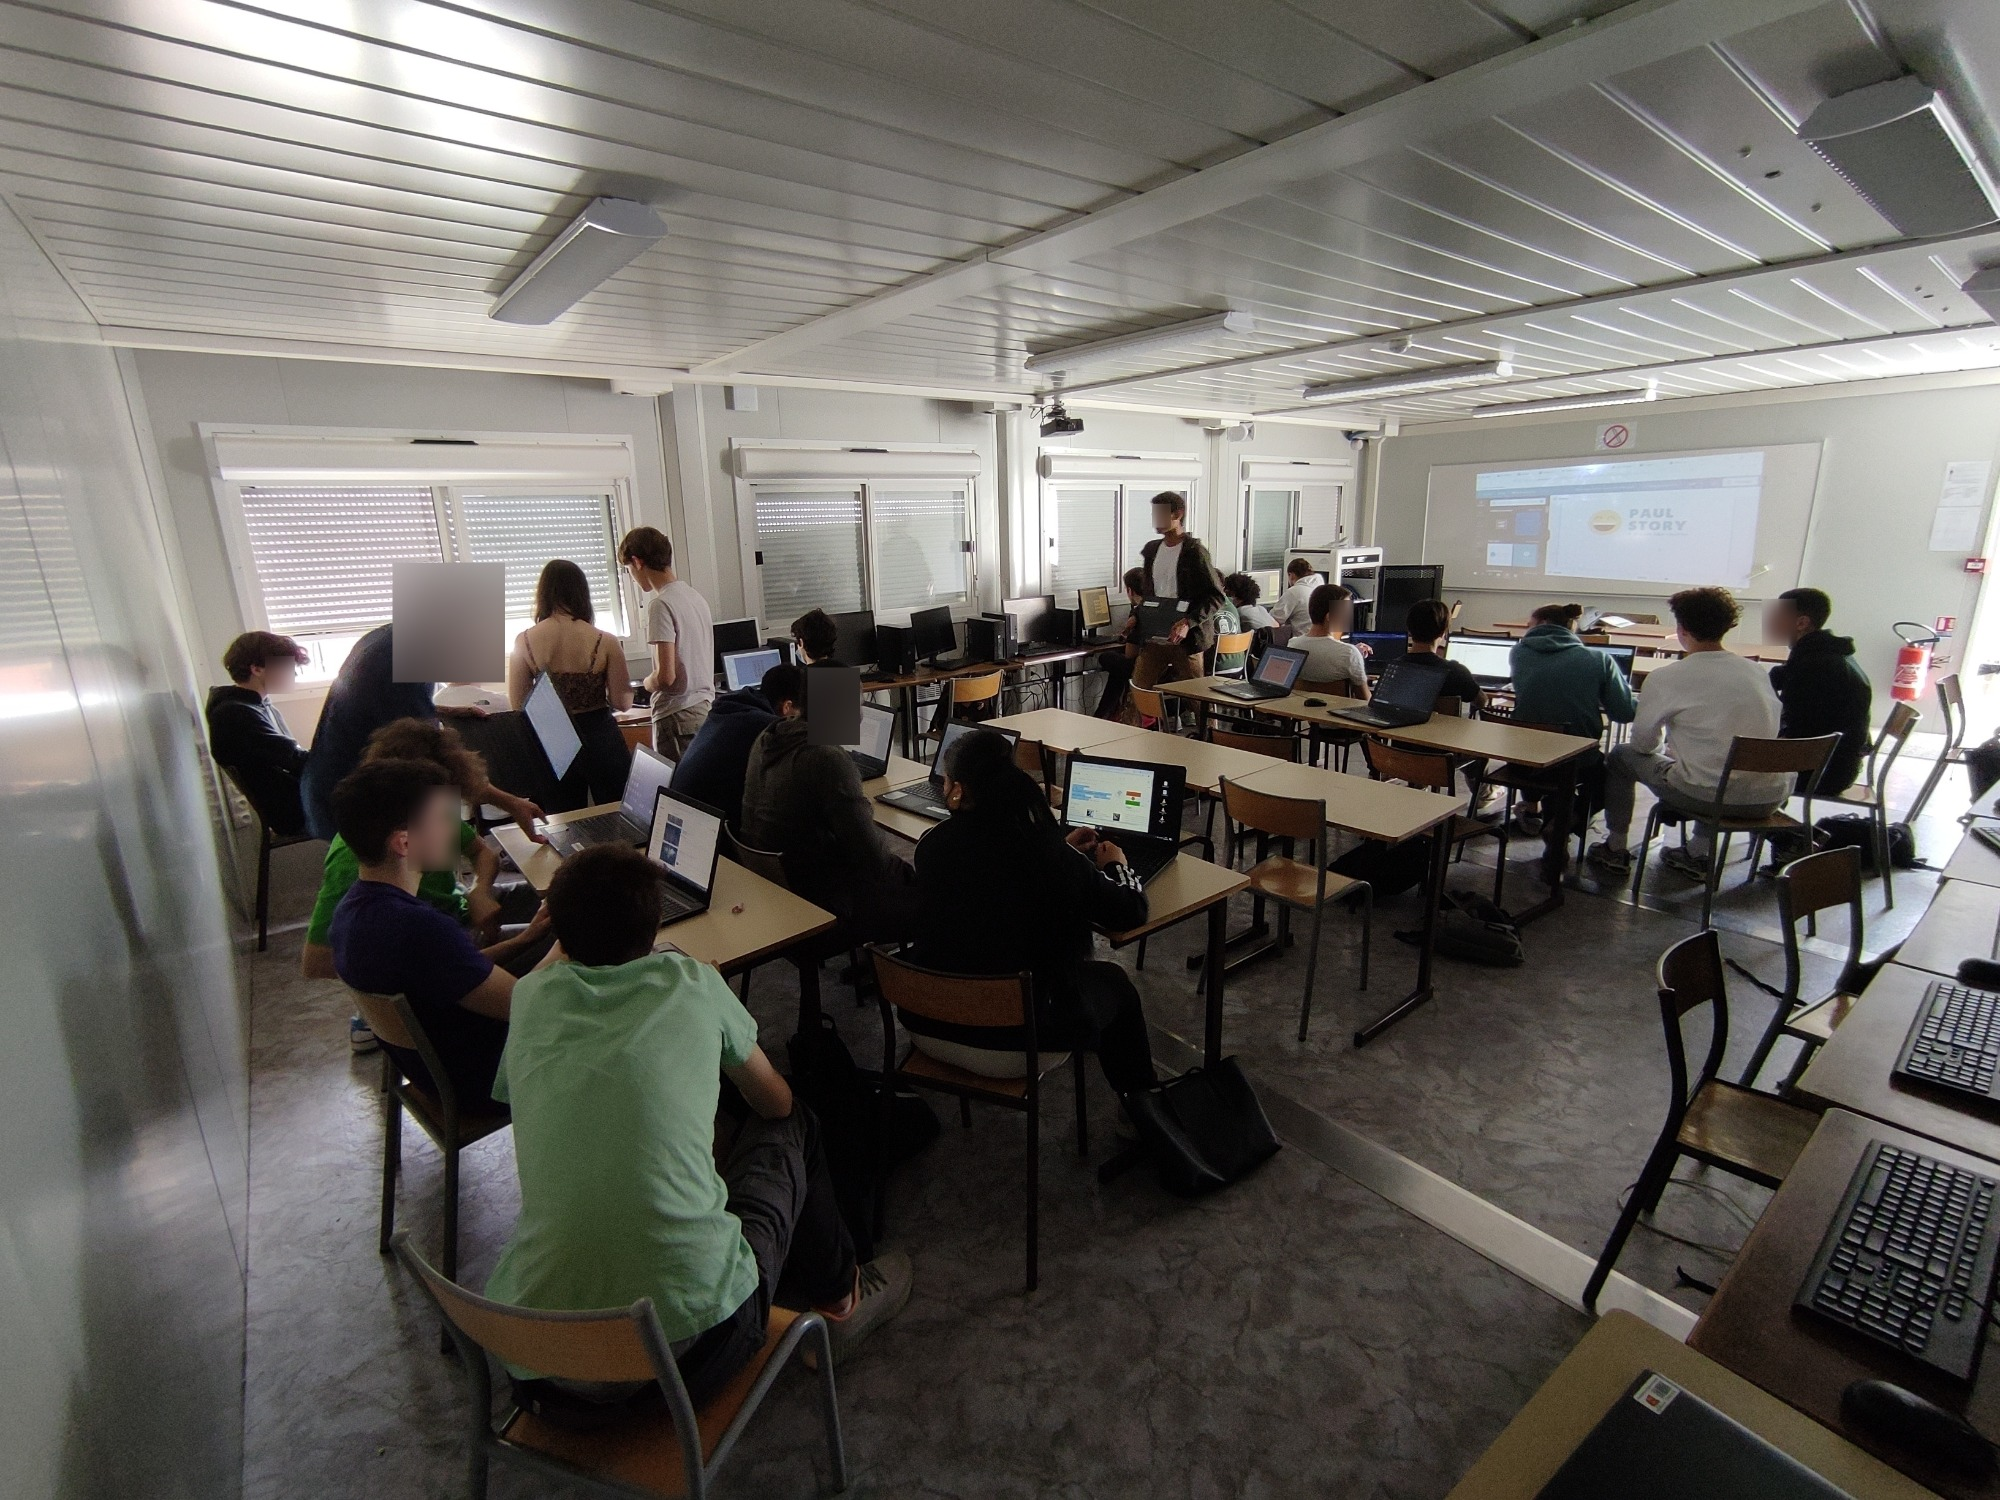
\includegraphics[width=0.8\textwidth]{annexes/pedagogiques/productions/jeux-photo-etudiants (1).jpg}
    \caption{Équipes interdisciplinaires en session de travail collaboratif (visages floutés pour l'anonymat).}
    \label{fig-equipes-travail-1}
\end{figure}

\subsection{Le défi humain : recruter et fédérer dans un contexte difficile}

Le recrutement des collègues a été particulièrement difficile dans un lycée d'élite où la culture de la collaboration bénévole était peu présente et où les emplois du temps étaient déjà très chargés.

\subsubsection{Stratégies de mobilisation développées}

\begin{enumerate}[leftmargin=*]
    \item \textbf{Communication ciblée} : présentation individualisée du projet à chaque collègue potentiel, en mettant en avant les bénéfices pour sa discipline
    \item \textbf{Limitation de l'engagement} : proposition d'un cadre horaire raisonnable (4 séances de 2h par enseignant)
    \item \textbf{Soutien institutionnel} : appui de ma tutrice INSPÉ auprès de la direction pour valoriser le projet
    \item \textbf{Valorisation des productions} : engagement à présenter le jeu dans chaque classe participante
\end{enumerate}

Cette expérience illustre la compétence \textbf{« Situer ses interventions dans un écosystème professionnel »} du référentiel MEEF \parencite{rncp38152}, compétence qui ne se limite pas à collaborer ponctuellement mais implique de créer et d'animer une dynamique collective \parencite{competences_transversales_eurecia}.

\subsection{Management de projet agile adapté au contexte scolaire}

J'ai adopté une posture de \textbf{tuteur-cadre} plutôt que de chef de projet direct, inspirée des méthodes agiles Scrum \parencite{scrum_education}. Cette approche développe l'autonomie des élèves dans la gestion de leur projet.

\subsubsection{Structure de management mise en place}

\begin{itemize}[leftmargin=*]
    \item \textbf{Réunions de lancement} : définition collective des objectifs, du planning et des rôles
    \item \textbf{Sprints de 2 semaines} : cycles de travail avec objectifs précis
    \item \textbf{Stand-up meetings} : points réguliers de 15 minutes en fin de séance
    \item \textbf{Rétrospectives} : bilans collectifs après chaque sprint pour ajuster l'organisation
    \item \textbf{Outils collaboratifs} : utilisation de Trello pour la gestion des tâches et de GitLab pour le versionnage du code
\end{itemize}

Cette organisation responsabilise les élèves et leur permet de développer des compétences de gestion de projet directement transférables au monde professionnel \parencite{projet_travail_groupe}.

\section{Axe 3 : Déroulement et défis rencontrés}

\subsection{Chronologie du projet}

\textbf{Septembre - Octobre} : Conception du moteur de jeu et recrutement des équipes\\
\textbf{Novembre - Décembre} : Premier sprint (définition du scénario, premiers graphismes)\\
\textbf{Janvier - Février} : Deuxième sprint (développement des niveaux, musiques)\\
\textbf{Mars - Avril} : Troisième sprint (traductions, tests, corrections)\\
\textbf{Mai} : Finalisation et présentation aux classes participantes

\subsection{Gestion réaliste des contraintes}

Comme tout projet ambitieux, celui-ci a connu plusieurs défis \parencite{projet_travail_groupe,competences_transversales} :

\subsubsection{Dépassement des délais initiaux}
Le planning initial prévoyait une finalisation en mars, mais des difficultés techniques (bugs complexes, incompatibilités entre modules) et organisationnelles (absences, examens blancs) ont imposé un report à mai. Cette gestion de l'imprévu a nécessité :
\begin{itemize}[leftmargin=*]
    \item Une repriorisation des fonctionnalités (abandon de certaines fonctionnalités secondaires)
    \item Une réorganisation du planning avec des séances de travail supplémentaires volontaires
    \item Une communication transparente avec tous les acteurs sur les ajustements nécessaires
\end{itemize}

\subsubsection{Fluctuation de l'implication}
Certains membres se sont moins investis que d'autres, nécessitant des interventions de médiation et de remotivation. Ces compétences de management relationnel, développées en entreprise \parencite{knowles_andragogy}, se sont révélées directement transférables au contexte pédagogique.



\section{Axe 4 : Résultats et Analyse Réflexive}

\subsection{Bilan des productions et impacts}

\subsubsection{Un produit fini complet et professionnel}

Le résultat final est un jeu de type Zelda 2D, fonctionnel et riche, comprenant \parencite{pygame_tutorial} :

\begin{itemize}[leftmargin=*]
    \item \textbf{4 niveaux jouables} avec difficulté progressive
    \item \textbf{Un scénario à message positif} : « La rédemption d'un homme riche » (thématique sociale proposée par les élèves)
    \item \textbf{Des énigmes variées} : logique, exploration, résolution de problèmes
    \item \textbf{Des objets à collecter} et un système d'inventaire
    \item \textbf{Des PNJ avec dialogues} contextuels et aide au joueur
    \item \textbf{Une bande sonore originale} composée spécifiquement pour le jeu
    \item \textbf{Une interface multilingue} (français, anglais, italien)
    \item \textbf{Un système de sauvegarde} permettant de reprendre la partie
\end{itemize}

\begin{figure}[H]
    \centering
    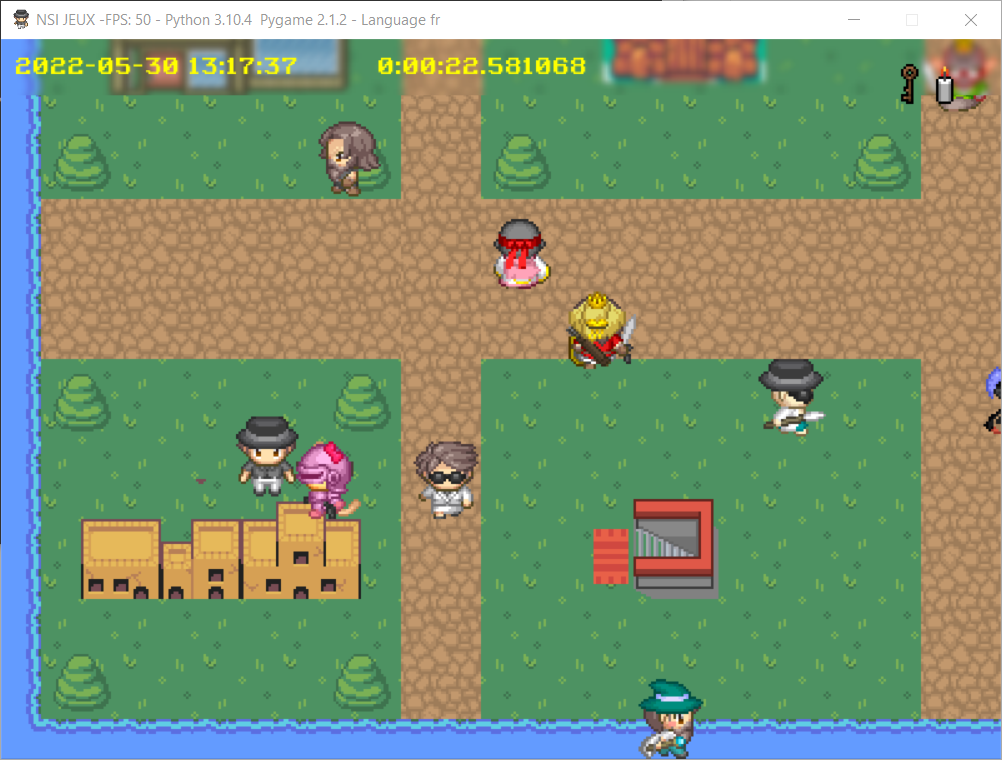
\includegraphics[width=0.8\textwidth]{annexes/pedagogiques/productions/jeux-capture-ecran (1).png}
    \caption{Interface principale du jeu développé collectivement.}
    \label{fig-jeu-menu}
\end{figure}

\begin{figure}[H]
    \centering
    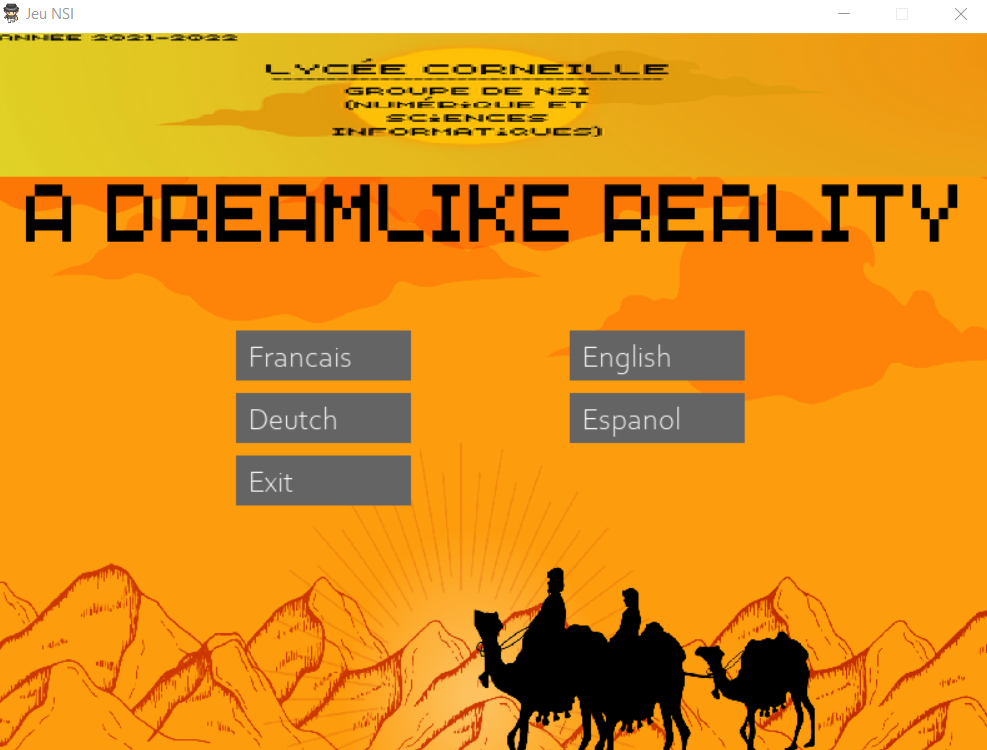
\includegraphics[width=0.8\textwidth]{annexes/pedagogiques/productions/jeux-capture-ecran (2).png}
    \caption{Exemple de niveau de jeu avec l'interface utilisateur.}
    \label{fig-jeu-niveau}
\end{figure}

\subsubsection{Impact au-delà de la classe}

Le projet a eu un rayonnement significatif \parencite{pedagogie_active} :

\begin{enumerate}[leftmargin=*]
    \item \textbf{Démonstrations dans les classes} : présentation du jeu dans toutes les classes des enseignants participants, valorisant le travail des élèves
    \item \textbf{Présentation en conseil pédagogique} : le projet a été présenté comme exemple de collaboration interdisciplinaire
    \item \textbf{Article dans le journal du lycée} : mise en valeur du travail collectif
    \item \textbf{Mise à disposition du jeu} : téléchargement possible sur la Forge des Communs Numériques Éducatifs \parencite{forge_educative}
\end{enumerate}

\subsubsection{Développement de compétences transversales}

L'évaluation qualitative post-projet révèle des acquis significatifs \parencite{competences_transversales_eurecia} :

\begin{itemize}[leftmargin=*]
    \item \textbf{Compétences techniques NSI} : Tous les élèves de l'équipe coordinatrice ont validé les compétences du programme relatives à la POO et à la gestion de projet
    \item \textbf{Compétences collaboratives} : 85\% des élèves déclarent avoir développé leur capacité à travailler en équipe interdisciplinaire
    \item \textbf{Autonomie et initiative} : 90\% des élèves déclarent avoir pris des initiatives personnelles dans le projet
    \item \textbf{Gestion du temps} : 75\% déclarent avoir amélioré leur capacité à respecter des délais
\end{itemize}

\subsubsection{Modalités d'évaluation}
L'évaluation du projet s'est appuyée sur une grille critériée permettant d'apprécier à la fois les compétences techniques et les compétences transversales.

\begin{longtable}{|p{3.5cm}|p{2.5cm}|p{2.5cm}|p{2.5cm}|p{2.5cm}|}
\caption{Grille d'évaluation Projet Collaboratif Interdisciplinaire - Jeu Vidéo} \\
\hline
\textbf{Compétences} & \textbf{Non acquis (0-7)} & \textbf{En cours (8-12)} & \textbf{Acquis (13-16)} & \textbf{Maîtrisé (17-20)} \\
\hline
\endfirsthead
\hline
\textbf{Compétences} & \textbf{Non acquis (0-7)} & \textbf{En cours (8-12)} & \textbf{Acquis (13-16)} & \textbf{Maîtrisé (17-20)} \\
\hline
\endhead

\textbf{Programmation Python/Pygame} &
Code non fonctionnel, erreurs majeures &
Code partiellement fonctionnel &
Code fonctionnel et structuré &
Code optimisé, commenté, élégant \\
\hline

\textbf{Collaboration interdisciplinaire} &
Travail en silo, pas d'échanges &
Échanges ponctuels &
Collaboration effective régulière &
Synergie créative, leadership \\
\hline

\textbf{Gestion de projet} &
Pas de planification &
Planning basique suivi &
Gestion efficace des tâches &
Méthodes agiles maîtrisées \\
\hline

\textbf{Intégration des 5 disciplines} &
Une seule discipline intégrée &
2-3 disciplines présentes &
4-5 disciplines harmonieusement intégrées &
Synergie exceptionnelle entre toutes les disciplines \\
\hline

\end{longtable}

\subsection{Analyse réflexive approfondie}

\subsubsection{Analyse a priori : Le pari de l'interdisciplinarité}
Mon intention pédagogique initiale reposait sur le postulat que le \textbf{jeu vidéo} agirait comme un "objet-frontière" \parencite{star_griesemer_boundary_objects}, capable de fédérer des disciplines cloisonnées (Arts, Langues, Histoire, Info). Je faisais l'hypothèse que :
\begin{itemize}
    \item La motivation intrinsèque pour le jeu vidéo compenserait la difficulté de la coordination.
    \item Les élèves développeraient naturellement des compétences de communication pour faire dialoguer leurs expertises respectives.
    \item Le rôle de "tuteur-cadre" suffirait à maintenir la cohésion sans interventionnisme excessif.
\end{itemize}

\subsubsection{Analyse a posteriori : La réalité du terrain}
L'expérience a validé la puissance motivationnelle du support, mais a révélé que la \textbf{collaboration ne se décrète pas}, elle s'apprend. J'ai observé que sans une structuration très forte (les rituels agiles), les groupes tendaient naturellement à travailler en silos (les graphistes font des dessins, les codeurs codent, sans se parler). La "magie" de l'interdisciplinarité n'a opéré que parce qu'elle a été provoquée et maintenue par une ingénierie de projet rigoureuse.

\subsubsection{Difficultés imprévues et régulations (Analyse Multi-agenda)}
La gestion de ce projet a nécessité une régulation fine de mon activité, analysable via le \textbf{multi-agenda de Bucheton} \parencite{bucheton_postures}. J'ai dû gérer simultanément des préoccupations parfois contradictoires :

\begin{itemize}[leftmargin=*]
    \item \textbf{Pilotage et Chronogenèse} : Contrairement à un cours magistral, le pilotage s'est fait « à vue ». J'ai dû accepter de relâcher le contrôle temporel strict pour m'adapter au rythme d'avancement disparate des groupes, acceptant que tous n'atteignent pas le même point au même moment.
    \item \textbf{Atmosphère et Tissage} : L'enjeu était de maintenir une atmosphère de travail collaboratif (bruit productif) tout en évitant la dispersion. Le tissage s'est opéré en reliant constamment leurs problèmes techniques immédiats (« mon personnage ne saute pas ») aux concepts théoriques vus en cours (« c'est une question de vecteur vitesse »).
    \item \textbf{Étayage et Postures} : Ma posture dominante a glissé du \textbf{contrôle} (au début) à l'\textbf{accompagnement} et au \textbf{lâcher-prise}. J'ai agi comme une « personne ressource », intervenant à la demande pour débloquer une situation (étayage local) plutôt que pour diriger l'action (étayage global).
\end{itemize}

Face aux obstacles spécifiques :
\begin{itemize}[leftmargin=*]
    \item \textbf{Hétérogénéité technique} : L'écart de niveau NSI 1ère/Terminale a menacé de bloquer le développement.
    \item \textbf{Solution} : Mise en place de "binômes de compétences" (tutorat par les pairs) et création de modules de code "prêts à l'emploi" pour les novices.
    
    \item \textbf{Tensions interpersonnelles} : Des conflits de leadership sont apparus.
    \item \textbf{Solution} : Médiation active et rappel des rôles définis par la charte de projet initiale.
    
    \item \textbf{Essoufflement de la motivation} : Baisse de régime au milieu du 2ème trimestre.
    \item \textbf{Solution} : Organisation d'une "démo intermédiaire" valorisante devant le Proviseur pour relancer la dynamique.
\end{itemize}

\subsubsection{Axes d'amélioration}
Pour une future itération, je proposerais :
\begin{itemize}
    \item \textbf{Une échelle plus réduite} : Commencer par un "Game Jam" de 48h pour souder les équipes avant le projet long.
    \item \textbf{Des outils de communication unifiés} : Imposer un seul canal (ex: Discord éducatif ou Teams) pour éviter la dispersion de l'information.
    \item \textbf{Une évaluation par les pairs formalisée} : Intégrer plus tôt la méthode de "notation à l'enveloppe" (voir Expérience 3) pour réguler l'investissement individuel.
\end{itemize}

\subsection{Transférabilité et compétences MEEF validées}

Cette expérience valide plusieurs blocs du référentiel RNCP38152 \parencite{rncp38152} à un niveau expert :

\subsubsection{BC09 - Acteur de la communauté éducative}

Je n'ai pas seulement collaboré, j'ai \textbf{initié et construit} une collaboration interdisciplinaire dans un environnement a priori peu favorable. Mobiliser des collègues agrégés de disciplines variées autour d'un projet numérique démontre des compétences avancées de :
\begin{itemize}[leftmargin=*]
    \item Leadership pédagogique
    \item Communication institutionnelle
    \item Diplomatie et négociation
    \item Animation d'une communauté éducative \parencite{competences_transversales}
\end{itemize}

\subsubsection{BC05 - Didactique de l'informatique et pédagogie de projet}

Cette expérience est un cas d'école de la pédagogie de projet \parencite{kilpatrick_project_method,dewey_experience_education,projet_methode_tlem}. Les notions techniques de NSI ne sont pas apprises hors-sol, mais au service d'un but créatif et motivant. La création du moteur de jeu constitue une forme avancée de transposition didactique : rendre appropriable par des lycéens un système informatique complexe \parencite{chevallard_transposition}.

\subsubsection{BC04 - Conduite de projet et recherche-action}

La démarche suivie (Analyse du problème → Conception d'une solution → Mise en œuvre → Analyse des résultats) est celle d'un praticien-chercheur \parencite{schon_reflective_practitioner,recherche_action_education}. Cette recherche-action illustre la conduite autonome d'un projet pédagogique complexe.

\subsubsection{BC06 - Praticien réflexif}

Mon rôle de tuteur-cadre et la mise en place d'une structure de management inspirée des méthodes agiles montrent que ma réflexion portait sur l'\textbf{organisation de l'apprentissage elle-même} \parencite{perrenoud_pratique_reflexive}, développant chez les élèves des compétences de gestion de projet essentielles pour leur future vie professionnelle \parencite{competences_transversales,scrum_education}.

\subsection{Perspectives de recherche}

Cette expérience nourrit directement mon projet de thèse sur plusieurs aspects \parencite{intelligence_artificielle_education} :

\begin{enumerate}[leftmargin=*]
    \item \textbf{IA et différenciation} : Comment l'IA pourrait-elle aider à adapter automatiquement les tâches du projet au niveau de chaque élève ?
    \item \textbf{Évaluation des compétences transversales} : Comment mesurer objectivement le développement des soft skills dans un projet collaboratif ?
    \item \textbf{Collaboration numérique} : Quels outils numériques optimisent la collaboration interdisciplinaire en contexte scolaire ?
\end{enumerate}
